\section{Privacy Preservation Analysis}
\label{sec:privacy}

\subsection{Privacy guarantees}

Within \Sys, potential privacy compromises arise if either the central, utility server or a malicious client can infer specific details about individual clients' logs, such as the applications in use or particular attributes like filenames and IP addresses. For each of the three components we present the proofs with strong privacy guarantees below:

\renewcommand{\thetheorem}{\arabic{theorem}}

\begin{theorem}[Central Server Privacy]
    For any two provenance graphs \(PGClient_1\), \(PGClient_2\) that differ only in the inclusion of a single node \(x\) and its \(\ell\)-hop attributed neighborhood (i.e., the local subgraph centered at \(x\), including all nodes in \(\mathcal{N}_\ell(x)\), edges, and associated attributes), the probability that an adversary \(\mathcal{A}\), observing only the GNN model updates received by the central server, can determine which graph was used deviates from random guessing by at most a negligible function \(\epsilon(n)\), where \(n\) is the security parameter representing the randomness complexity of the client-side training process.
    \end{theorem}
    
    \begin{proof}
    Let \(x \in \mathcal{V}_i\) denote a node in the client provenance graph \(PGClient_i = (\mathcal{V}_i, \mathcal{E}_i)\). Define its \(\ell\)-hop attributed neighborhood as the induced subgraph that includes:
    - the node \(x\),
    - all nodes within \(\ell\) hops (i.e., \(\mathcal{N}_\ell(x)\)),
    - all edges between them, and
    - their associated node and edge attributes.
    
    Let \(PGClient_1\) and \(PGClient_2\) be two graphs that are identical except that \(PGClient_1\) includes node \(x\) and its \(\ell\)-hop attributed neighborhood, while \(PGClient_2\) does not.
    
    Each client transforms the contextual attributes using the harmonized embedding model \(M_{\text{w2v-harm}}\), which produces vector representations for both nodes and edges. These embeddings are input to an ensemble of category-specific GNNs \(\{GNN_1, \ldots, GNN_{K_{\text{cat}}}\}\), each trained independently on its category. The resulting local gradient updates are sent to the central server, where they are aggregated into global model weights \(w_j^{(r)}\) for each category \(j\).
    
    Let \(GNN_j(PGClient_i; r)\) denote the client-side training of submodel \(j\) on provenance graph \(PGClient_i\) using randomness seed \(r\), which controls embedding initialization, mini-batch sampling, and optimizer dynamics. Even for the same graph, different runs may yield different model updates due to this local randomness.
    
    Let \(P_1\) and \(P_2\) denote the distributions over model updates resulting from training on \(PGClient_1\) and \(PGClient_2\), respectively. Their statistical distance is defined as:
    \begin{align*}
    \Delta(P_1, P_2) = \sup_{S} \big|\, 
    & \Pr\big[GNN_j(PGClient_1) \in S\big] \\
    & - \Pr\big[GNN_j(PGClient_2) \in S\big] \,\big|,
    \end{align*}
    where the supremum is taken over all measurable subsets \(S\) of the update space.
    
    Even though the only change between the graphs is node \(x\), the message-passing nature of GNNs causes its \(\ell\)-hop neighbors to also influence and be influenced by the presence of \(x\). Since embeddings propagate through the graph, the resulting update signal is not isolated to \(x\), but distributed across the receptive field. This non-locality, coupled with random initialization and category-specific GNNs, makes the change statistically hard to detect.
    
    Additionally, the number of possible attributed neighborhoods grows exponentially. Given node attribute vocabulary \(\mathcal{A}_v\) and edge attribute vocabulary \(\mathcal{A}_e\), the number of candidate neighborhoods centered at \(x\) satisfies:
    \[
    |\mathcal{S}(x)| \in \mathcal{O}\left(|\mathcal{A}_v|^{|\mathcal{N}_\ell(x)|} \cdot |\mathcal{A}_e|^{|\mathcal{N}_\ell(x)|}\right).
    \]
    Thus, an adversary attempting to infer the presence of \(x\) would need to simulate an exponential number of structurally and semantically plausible neighborhoods, without access to the embedding function \(M_{\text{w2v-harm}}\) or the client’s randomness seed.
    
    Consequently, the adversary's distinguishing advantage is bounded by:
    \[
    \left| \Pr[\mathcal{A}(w_j^{(r)} \text{ from } PGClient_1) = 1] - \tfrac{1}{2} \right| \leq \epsilon(n),
    \]
    where \(\epsilon(n)\) is negligible in the security parameter \(n\). That is, for every polynomial \(p(n)\), there exists \(n_0\) such that for all \(n > n_0\), \(\epsilon(n) < \frac{1}{p(n)}\).
    
    Therefore, \Sys ensures indistinguishability-based privacy under server-side observation of GNN model updates, even when client graphs differ by a single node and its attributed neighborhood.
    \end{proof}
    
\begin{theorem}[Utility Server Privacy]
Let \(M_{\text{w2v-harm}}: \mathcal{P}_{\text{global}} \to \mathbb{R}^d\) denote the client-side embedding function that maps input tokens \(p \in \mathcal{P}_{\text{global}}\) to high-dimensional vectors \(e \in \mathbb{R}^d\). In \Sys, each client independently applies \(M_{\text{w2v-harm}}\) to locally generate semantic embeddings and encrypts all tokens before transmission. The utility server receives only encrypted tokens and their corresponding embeddings. Then, for any embedding \(e\) observed by the utility server, the probability that an adversary \(\mathcal{A}\) can correctly identify the original token \(p\) such that \(e = M_{\text{w2v-harm}}(p)\) is at most \(\frac{1}{|\mathcal{P}_{\text{global}}|} + \epsilon(d)\), where \(\epsilon(d)\) is negligible in the embedding dimension \(d\).
\end{theorem}

\begin{proof}
Each client applies the local embedding function \(M_{\text{w2v-harm}}\) to convert input tokens \(p \in \mathcal{P}_{\text{global}}\) into semantic vectors \(e = M_{\text{w2v-harm}}(p) \in \mathbb{R}^d\), and encrypts the original tokens before sending them to the utility server. Thus, the utility server receives only encrypted identifiers and their associated semantic embeddings, with no access to the plaintext tokens or the internals of \(M_{\text{w2v-harm}}\).

The embedding function \(M_{\text{w2v-harm}}\), trained using a distributional objective (e.g., skip-gram with negative sampling), is inherently non-injective. Its goal is to preserve contextual similarity, not one-to-one invertibility. Formally, there exist distinct tokens \(p_1, p_2 \in \mathcal{P}_{\text{global}}\), with \(p_1 \neq p_2\), such that \(M_{\text{w2v-harm}}(p_1) \approx M_{\text{w2v-harm}}(p_2)\). Consequently, the preimage set of a given embedding \(e\) is:
\[
M_{\text{w2v-harm}}^{-1}(e) = \{p \in \mathcal{P}_{\text{global}} \mid M_{\text{w2v-harm}}(p) \approx e\},
\]
which may contain multiple semantically related tokens. This ambiguity arises because \(M_{\text{w2v-harm}}\) typically involves non-linear transformations and dimensionality reduction.

Let \(\text{Rev}(M_{\text{w2v-harm}}, e)\) denote a hypothetical reverse function attempting to infer \(p\) from \(e\). Since the utility server has no access to the original training data or encryption keys, its best strategy is effectively bounded by random guessing:
\[
\Pr[\text{Rev}(M_{\text{w2v-harm}}, e) = p] \leq \frac{1}{|\mathcal{P}_{\text{global}}|} + \epsilon(d),
\]
where \(\epsilon(d)\) becomes negligible as \(d\) increases. That is, for every polynomial \(p(d)\), there exists \(d_0\) such that for all \(d > d_0\), \(\epsilon(d) < \frac{1}{p(d)}\).

Therefore, \Sys guarantees that the probability of reverse-engineering semantic embeddings at the utility server is negligible, ensuring strong semantic privacy.
\end{proof}

\begin{theorem}[Client-Level Privacy]
Let \(w_j^{(r)}\) be the global model weights obtained by aggregating updates from clients \(\mathcal{C} = \{C_1, C_2, \ldots, C_N\}\), where each client observes only a disjoint subset of application-specific semantic attribute vectors. Suppose a malicious client \(C_{\text{adv}} \in \mathcal{C}\) attempts to infer whether a particular token \(p \in \mathcal{P}_{\text{global}}\) used by another client is present in the global model. Then, under standard aggregation (e.g., FedAvg) and semantic vector disjointness across clients, the probability that \(C_{\text{adv}}\) can infer the presence of \(p\) is bounded by:
\[
\Pr[\text{Infer}(w_j^{(r)}, p) = 1] \leq \frac{|\mathcal{P}_{\text{adv}}|}{|\mathcal{P}_{\text{global}}|} + \epsilon(m),
\]
where \(\mathcal{P}_{\text{adv}}\) is the set of tokens accessible to \(C_{\text{adv}}\), and \(\epsilon(m)\) is negligible in the number of disjoint-contributing clients \(m = |\mathcal{P}_{\text{global}} \setminus \mathcal{P}_{\text{adv}}|\).
\end{theorem}

\begin{proof}
The global model \(w_j^{(r)}\) is constructed via aggregation of updates from clients \(\mathcal{C}\), each of which trains a local GNN ensemble using embeddings from their private token subset. Let \(\mathcal{P}_{\text{global}}\) denote the full vocabulary and \(\mathcal{P}_{\text{adv}} \subset \mathcal{P}_{\text{global}}\) the subset observed by adversarial client \(C_{\text{adv}}\).

Client \(C_{\text{adv}}\) observes \(w_j^{(r)}\), which encodes aggregated signals from all participating clients. However, without access to \(M_{\text{w2v-harm}}(p)\) for \(p \notin \mathcal{P}_{\text{adv}}\), the adversary cannot attribute any weight shifts to specific unseen tokens.

We model the inference as a binary decision: \(\text{Infer}(w_j^{(r)}, p) = 1\) if the adversary believes \(p\) is present. Since the adversary lacks semantic embeddings for tokens outside \(\mathcal{P}_{\text{adv}}\), its best strategy is random guessing over the unknown token space. Thus:
\[
\Pr[\text{Infer}(w_j^{(r)}, p) = 1] \leq \frac{|\mathcal{P}_{\text{adv}}|}{|\mathcal{P}_{\text{global}}|} + \epsilon(m),
\]
where \(\epsilon(m)\) accounts for statistical leakage from partial token overlaps. As \(m\) increases, \(\epsilon(m)\) becomes negligible.

\end{proof}

Therefore, the architecture of \Sys robustly defends against inference attacks from both servers and malicious clients. Its privacy guarantees rely on decentralized learning, semantic embedding ambiguity, and the assumption of non-colluding servers, as upheld by prior works~\cite{roy2020crypte,wu2022federated}.

\subsection{Effect of differential privacy on accuracy}
\label{app:dp}

In Section~\ref{sec:privacy}, we analyze how our system design offers strong guarantees against model inference attacks. Here we discuss another alternative technique for preserving privacy through the use of Differential Privacy (DP). It can be integrated with federated learning to protect against inference attacks~\cite{lyu2020threats,nasr2019comprehensive,zari2021efficient}, though it comes at the cost of detection accuracy.

Differential privacy safeguards the model by injecting a controlled amount of Gaussian noise into its parameters, thereby concealing the influence of any individual data point. In our work, we adopt a node-level DP strategy, which ensures that each node’s features and labels are protected when noise is added to the gradient updates. As a result, individual node contributions remain obscured in the aggregated model parameters, reducing the likelihood of identifying specific nodes or their features. We conduct experiments to examine how varying levels of differential privacy noise affect the detection performance of \Sys. The noise is adjusted based on a privacy budget defined by~$\epsilon$. This noise is applied to local \gnnshort model updates before they are aggregated at the central server during federated averaging, as described in Section~\ref{sec:methodology}.

\begin{figure}[!t]
  \centering
  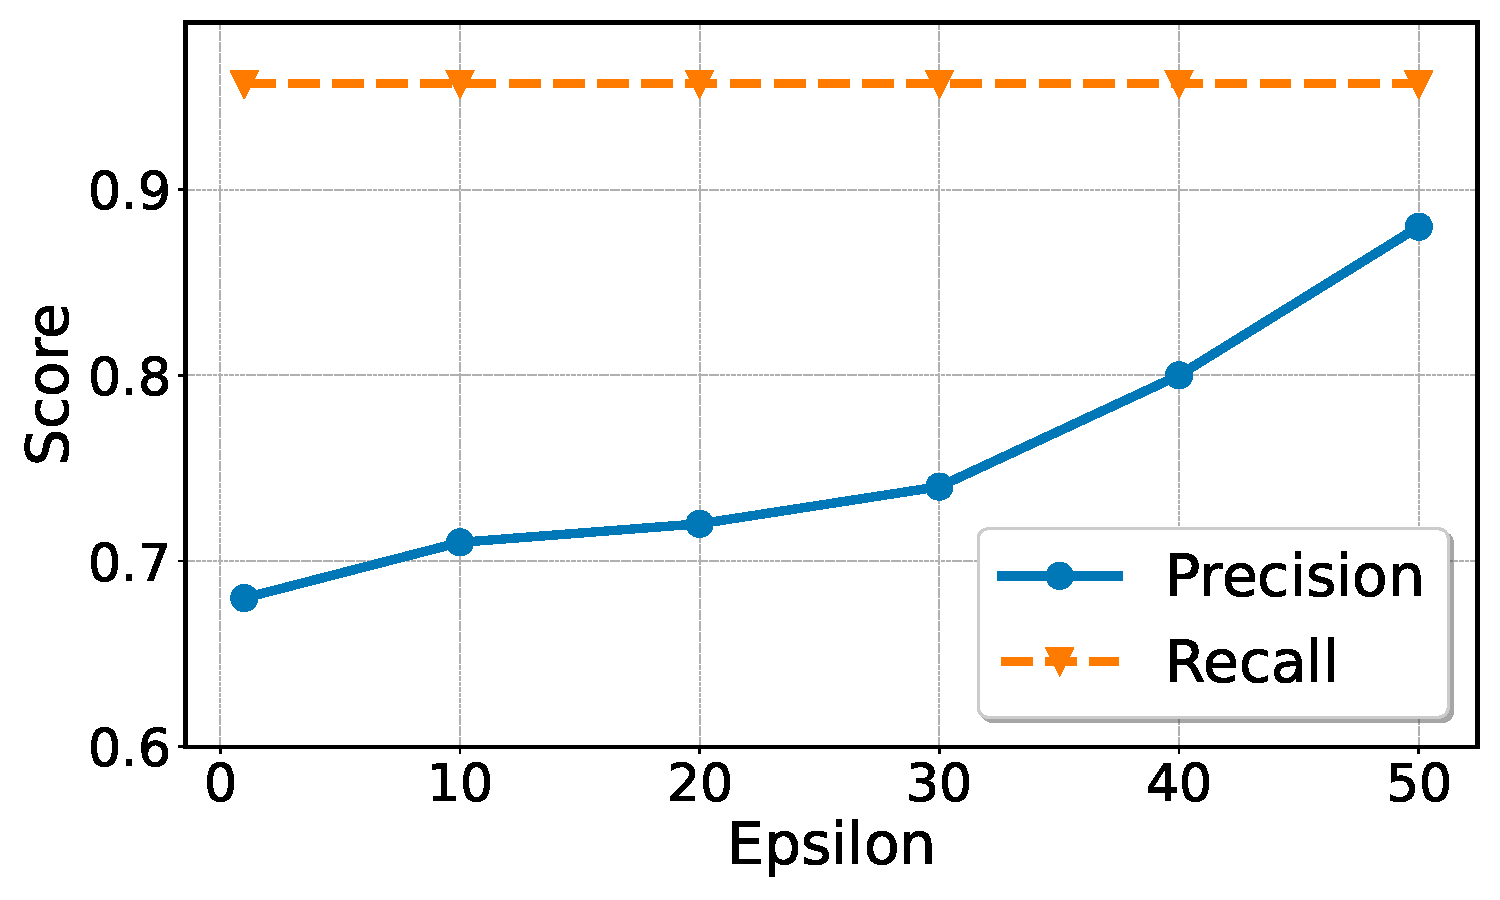
\includegraphics[width=0.3\textwidth]{fig/epsvsscore.pdf}
  \caption{Effect of differential privacy noise on detection using E3 dataset. Note that we observed similar results on the other datasets.}
  \label{epsvsscore}
  \vspace{-2ex}
\end{figure}


The privacy budget~$\epsilon$ plays a pivotal role. Lower values of $\epsilon$ increase the noise injected into the model, which enhances privacy at the expense of detection performance. Conversely, higher values of $\epsilon$ inject less noise, improving detection accuracy but offering weaker privacy guarantees. By tuning $\epsilon$ during training, we explore the balance between privacy and detection effectiveness across various settings. As shown in Figure~\ref{epsvsscore}, increasing the noise level (i.e., reducing $\epsilon$) degrades the model’s utility, thereby providing more privacy at the cost of lower accuracy.

Hence, although DP is a valid solution for protecting privacy, the accuracy deterioration that comes with it reduces its utility in the domain of intrusion detection, where high detection performance is needed. Due to these reasons, we do not use DP in \Sys and instead design a dual-server architecture to offer privacy guarantees without adding noise to the model updates.
